%%%%%%%%%%%%%%%%%%%%%%%%%%%%%%%%%%%%%%%%%%%%%%%%%%%%%%%%%%%%%%%%%%%%%%%%%%%%%%%%%%
\begin{frame}[fragile]\frametitle{}

\begin{center}
{\Large Introduction to spaCy}

{\tiny (Ref: https://spacy.io/usage/spacy-101)}

\end{center}


\end{frame}
%

%%%%%%%%%%%%%%%%%%%%%%%%%%%%%%%%%%%%%%%%%%%%%%%%%%%%%%%%%%%%%%%%%%%%%%%%%%%%%%%%%%
\begin{frame}[fragile]\frametitle{What is spaCy?}
  \begin{itemize}
    \item spaCy is a free, open-source library for advanced Natural Language Processing (NLP) in Python.
		\item Production ready.
		\item Used to build information extraction or natural language understanding systems, or to pre-process text for deep learning.
  \end{itemize}
	
\end{frame}



%%%%%%%%%%%%%%%%%%%%%%%%%%%%%%%%%%%%%%%%%%%%%%%%%%%%%%%%%%%%%%%%%%%%%%%%%%%%%%%%%%
\begin{frame}[fragile]\frametitle{What spaCy isn't?}
  \begin{itemize}
    \item Not a platform or “an API” or software as a service, or a web application
		\item Not an out-of-the-box chat bot engine.
		\item Not research software.  It's built on the latest research, but it's designed to get things done.
		\item Not a company. It's an open-source library. Company's name is `Explosion AI'.
  \end{itemize}
	
\end{frame}

%%%%%%%%%%%%%%%%%%%%%%%%%%%%%%%%%%%%%%%%%%%%%%%%%%%%%%%%%%%%%%%%%%%%%%%%%%%%%%%%%%
\begin{frame}[fragile]\frametitle{Installation}
Based on OS, version, etc an installation command can be generated at https://spacy.io/usage

	
\begin{center}
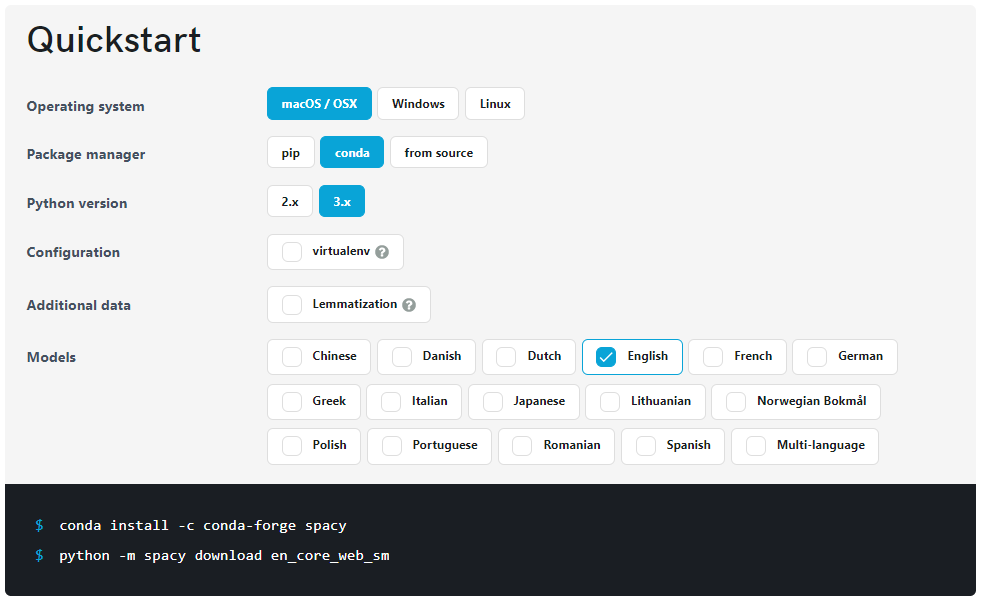
\includegraphics[width=0.8\linewidth,keepaspectratio]{spacy3}
\end{center}

\end{frame}

%%%%%%%%%%%%%%%%%%%%%%%%%%%%%%%%%%%%%%%%%%%%%%%%%%%%%%%%%%%%%%%%%%%%%%%%%%%%%%%%%%
\begin{frame}[fragile]\frametitle{Core Idea}
  \begin{itemize}
    \item Model object, typically called as `nlp' is the core object.
			\item Can use it like a function to analyze text.
		\item It contains processing pipeline
		\item It also includes language specific rules, say, for tokenization.
		\item You can either load it \lstinline|nlp = spacy.load('...')| or instantiate from existing class \lstinline|nlp = English()|
		\item `nlp' object after processing `text' produces `doc' object \lstinline|doc = nlp(text)|
		\item `doc' has all the text processing results stored
		\item `doc' can be instantiated also \lstinline|doc = Doc(nlp.vocab, words=words, spaces=spaces)|
		\item `span' object has multiple tokens. Its just a view and not actual data. \lstinline|span = doc[1:3]|
  \end{itemize}
	
\begin{center}
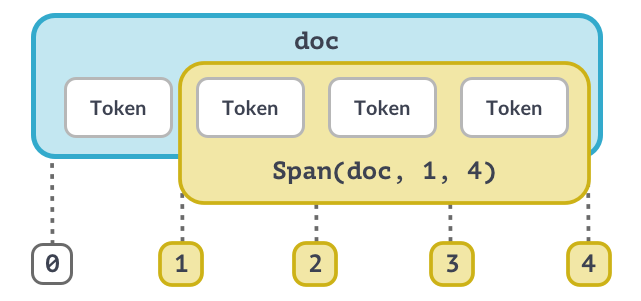
\includegraphics[width=0.5\linewidth,keepaspectratio]{spacy17}
\end{center}

\end{frame}

%%%%%%%%%%%%%%%%%%%%%%%%%%%%%%%%%%%%%%%%%%%%%%%%%%%%%%%%%%%%%%%%%%%%%%%%%%%%%%%%%%
\begin{frame}[fragile]\frametitle{Exercise}

  \begin{itemize}
    \item Import the English class from spacy.lang.en and create the nlp object.
    \item Create a doc and print its text.
  \end{itemize}

  \begin{lstlisting}
from spacy.lang.____ import ____

nlp = ____

doc = nlp("This is a sentence.")

print(____.text)
  \end{lstlisting}

Extra: Import the German class from spacy.lang.de and create the nlp object and use it on ``Ich liebe!''

\end{frame}

%%%%%%%%%%%%%%%%%%%%%%%%%%%%%%%%%%%%%%%%%%%%%%%%%%%%%%%%%%%%%%%%%%%%%%%%%%%%%%%%%%
\begin{frame}[fragile]\frametitle{Exercise}

  \begin{itemize}
    \item Import the English language class and create the nlp object.
    \item Process the text and instantiate a Doc object in the variable doc.
    \item Select the first token of the Doc and print its text.
  \end{itemize}

  \begin{lstlisting}
from spacy.lang.____ import ____

nlp = ____

doc = nlp("I like tree kangaroos and narwhals.")

first_token = doc[____]

print(first_token.____)
  \end{lstlisting}
	
\end{frame}

%%%%%%%%%%%%%%%%%%%%%%%%%%%%%%%%%%%%%%%%%%%%%%%%%%%%%%%%%%%%%%%%%%%%%%%%%%%%%%%%%%
\begin{frame}[fragile]\frametitle{Best Practices}

  \begin{itemize}
    \item Doc and Span are very powerful and hold references and relationships of words and sentences
    \item Convert result to strings as late as possible. 
		\item If you do it too early, you'll lose all relationships between the tokens.
    \item Use token attributes if available – for example, \lstinline|token.i|  for the token index
    \item Don't forget to pass in the shared vocab
  \end{itemize}

\end{frame}


%%%%%%%%%%%%%%%%%%%%%%%%%%%%%%%%%%%%%%%%%%%%%%%%%%%%%%%%%%%%%%%%%%%%%%%%%%%%%%%%%%
\begin{frame}[fragile]\frametitle{Evaluate}

Whats wrong with following code?

  \begin{lstlisting}
import spacy

nlp = spacy.load("en_core_web_sm")
doc = nlp("Berlin looks like a nice city")

# Get all tokens and part-of-speech tags
token_texts = [token.text for token in doc]
pos_tags = [token.pos_ for token in doc]

for index, pos in enumerate(pos_tags):
    # Check if the current token is a proper noun
    if pos == "PROPN":
        # Check if the next token is a verb
        if pos_tags[index + 1] == "VERB":
            result = token_texts[index]
            print("Found proper noun before a verb:", result)
  \end{lstlisting}

\end{frame}

%%%%%%%%%%%%%%%%%%%%%%%%%%%%%%%%%%%%%%%%%%%%%%%%%%%%%%%%%%%%%%%%%%%%%%%%%%%%%%%%%
\begin{frame}[fragile]\frametitle{Assignment}


  \begin{itemize}
    \item Rewrite the code to use the native token attributes instead of lists of token\_texts and pos\_tags.
    \item Loop over each token in the doc and check the token.pos\_ attribute.
    \item Use doc[token.i + 1] to check for the next token and its .pos\_ attribute.
    \item If a proper noun before a verb is found, print its token.text.
  \end{itemize}

\end{frame}



%%%%%%%%%%%%%%%%%%%%%%%%%%%%%%%%%%%%%%%%%%%%%%%%%%%%%%%%%%%%%%%%%%%%%%%%%%%%%%%%%%
\begin{frame}[fragile]\frametitle{Solution}

  \begin{lstlisting}
import spacy

nlp = spacy.load("en_core_web_sm")
doc = nlp("Berlin looks like a nice city")

# Get all tokens and part-of-speech tags
token_texts = [token.text for token in doc]
pos_tags = [token.pos_ for token in doc]

for index, pos in enumerate(pos_tags):
    # Check if the current token is a proper noun
    if pos == "PROPN":
        # Check if the next token is a verb
        if pos_tags[index + 1] == "VERB":
            result = token_texts[index]
            print("Found proper noun before a verb:", result)
  \end{lstlisting}

\end{frame}

%%%%%%%%%%%%%%%%%%%%%%%%%%%%%%%%%%%%%%%%%%%%%%%%%%%%%%%%%%%%%%%%%%%%%%%%%%%%%%%%%%
\begin{frame}[fragile]\frametitle{Features}
\begin{center}
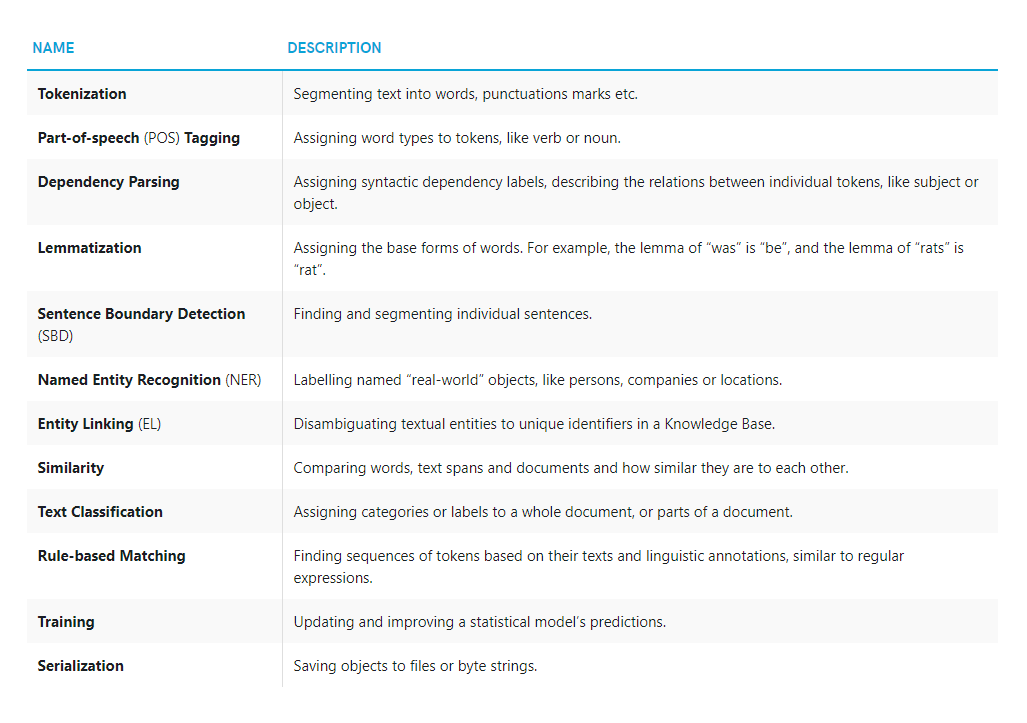
\includegraphics[width=0.8\linewidth,keepaspectratio]{spacy4}
\end{center}

\end{frame}



%%%%%%%%%%%%%%%%%%%%%%%%%%%%%%%%%%%%%%%%%%%%%%%%%%%%%%%%%%%%%%%%%%%%%%%%%%%%%%%%%%
\begin{frame}[fragile]\frametitle{How spaCy Works?}
  \begin{itemize}
    \item Example 1: ``Apple is looking at buying U.K. startup for \$1 billion''
		\item Example 2: ``Ishu ate the Apple''
		\item `Apple' in both the above examples is different. Can spaCy identify (named entity recognition) differently?
  \end{itemize}
	
\begin{center}
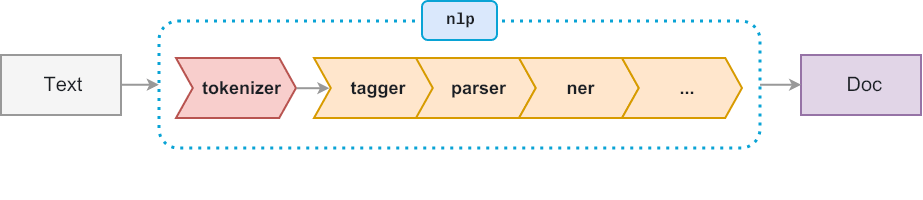
\includegraphics[width=0.8\linewidth,keepaspectratio]{spacy5}
\end{center}
	
\end{frame}

%%%%%%%%%%%%%%%%%%%%%%%%%%%%%%%%%%%%%%%%%%%%%%%%%%%%%%%%%%%%%%%%%%%%%%%%%%%%%%%%%%
\begin{frame}[fragile]\frametitle{Pre Trained models}
\begin{itemize}
\item Pre-trained models, like 'en\_core\_web\_sm', have various NLP sub components defined. `sm' is for small.
\item Similarly other models like  'en\_core\_web\_md' (medium) and 'en\_core\_web\_lg' (large) are some of the English models.
\item Similarly `de\_core\_news\_sm' (German) and  `es\_core\_news\_sm' (Spanish) are some other language models.
\end{itemize}

\begin{center}
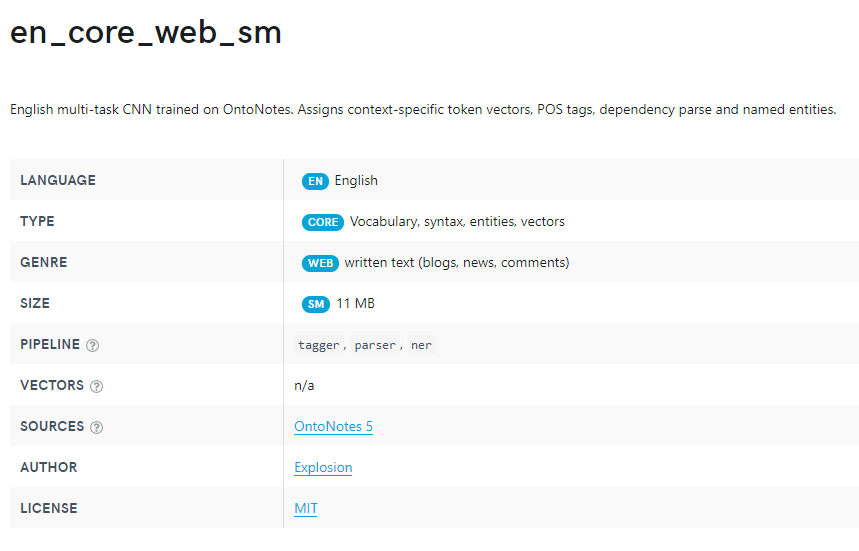
\includegraphics[width=0.6\linewidth,keepaspectratio]{spacy7}
\end{center}

\end{frame}


%%%%%%%%%%%%%%%%%%%%%%%%%%%%%%%%%%%%%%%%%%%%%%%%%%%%%%%%%%%%%%%%%%%%%%%%%%%%%%%%%%
\begin{frame}[fragile]\frametitle{spaCy Load under the hood}
  \begin{itemize}
    \item Easy to create own pipeline with reusable components.
		\item Includes spaCy's default tagger, parser and entity recognizer, but also your own custom processing functions.
		\item At loading a model, spaCy loos at meta.json
		\begin{lstlisting}
meta.json:
{
  "lang": "en",
  "name": "core_web_sm",
  "description": "Example model for spaCy",
  "pipeline": ["tagger", "parser", "ner"]
}
\end{lstlisting}

\item Iterate over the pipeline names and create each component using \lstinline|create_pipe|, which looks them up in Language.factories
\item Add each pipeline component to the pipeline in order, using \lstinline|add_pipe|

  \end{itemize}
	
	
\end{frame}

%%%%%%%%%%%%%%%%%%%%%%%%%%%%%%%%%%%%%%%%%%%%%%%%%%%%%%%%%%%%%%%%%%%%%%%%%%%%%%%%%%
\begin{frame}[fragile]\frametitle{Pipeline under the hood}
  \begin{itemize}
    \item When you call nlp on a text, spaCy will tokenize it and then call each component on the Doc, in order.
		\begin{lstlisting}
doc = nlp.make_doc("This is a sentence")   # create a Doc from raw text
for name, proc in nlp.pipeline:             # iterate over components in order
    doc = proc(doc)                         # apply each component

print(nlp.pipeline)
# [('tagger', <spacy.pipeline.Tagger>), ('parser', <spacy.pipeline.DependencyParser>), ('ner', <spacy.pipeline.EntityRecognizer>)]
print(nlp.pipe_names)
# ['tagger', 'parser', 'ner']
\end{lstlisting}

\item All components return the modified document, which is then processed by the component next in the pipeline.

  \end{itemize}
	
	
\end{frame}

%%%%%%%%%%%%%%%%%%%%%%%%%%%%%%%%%%%%%%%%%%%%%%%%%%%%%%%%%%%%%%%%%%%%%%%%%%%%%%%%%%
\begin{frame}[fragile]\frametitle{Built-in pipeline components}
\begin{center}
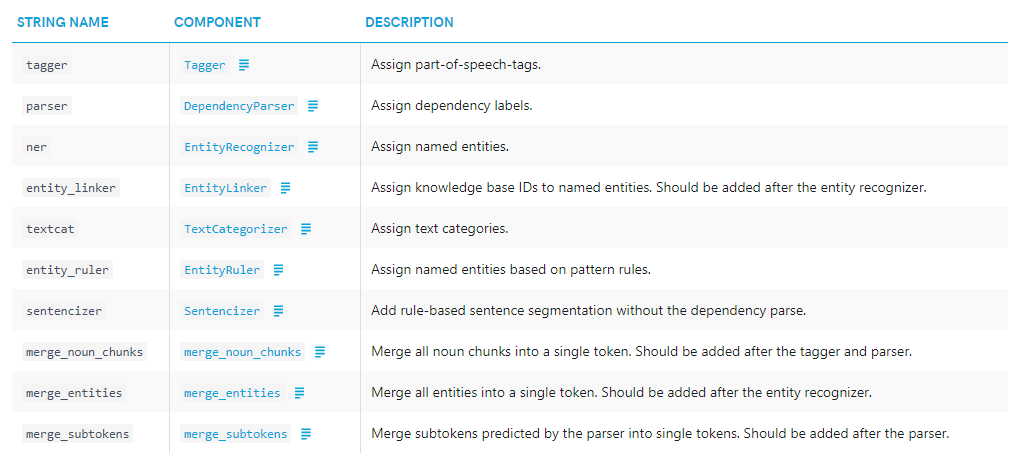
\includegraphics[width=\linewidth,keepaspectratio]{spacy10}
\end{center}

\end{frame}

%%%%%%%%%%%%%%%%%%%%%%%%%%%%%%%%%%%%%%%%%%%%%%%%%%%%%%%%%%%%%%%%%%%%%%%%%%%%%%%%%%
\begin{frame}[fragile]\frametitle{Disabling}
  \begin{itemize}
    \item If you don't need a particular component of the pipeline – for example, the tagger or the parser, you can disable loading it
		\begin{lstlisting}
nlp = spacy.load("en_core_web_sm", disable=["tagger", "parser"])
nlp = English().from_disk("/model", disable=["ner"])
\end{lstlisting}

\item If you only need a Doc object with named entities, there's no need to run all pipeline components on it
		\begin{lstlisting}
for doc in nlp.pipe(texts, disable=["tagger", "parser"]):
    # Do something with the doc here
\end{lstlisting}
  \end{itemize}
	
	
\end{frame}

%%%%%%%%%%%%%%%%%%%%%%%%%%%%%%%%%%%%%%%%%%%%%%%%%%%%%%%%%%%%%%%%%%%%%%%%%%%%%%%%%%
\begin{frame}[fragile]\frametitle{Custom Component}
  \begin{itemize}
    \item A component receives a Doc object and can modify it


\item  By adding a component to the pipeline, you'll get access to the Doc at any point during processing
  \end{itemize}
	
		\begin{lstlisting}
import spacy

def my_component(doc):
    print("After tokenization, this doc has {} tokens.".format(len(doc)))
    print("The part-of-speech tags are:", [token.pos_ for token in doc])
    if len(doc) < 10:
        print("This is a pretty short document.")
    return doc

nlp = spacy.load("en_core_web_sm")
nlp.add_pipe(my_component, name="print_info", last=True)
print(nlp.pipe_names)  # ['tagger', 'parser', 'ner', 'print_info']
doc = nlp("This is a sentence.")
\end{lstlisting}	
	
\end{frame}

%%%%%%%%%%%%%%%%%%%%%%%%%%%%%%%%%%%%%%%%%%%%%%%%%%%%%%%%%%%%%%%%%%%%%%%%%%%%%%%%%%
\begin{frame}[fragile]\frametitle{Custom Component Class}
You can also wrap your component as a class to allow initializing it with custom settings and hold state within the component. This is useful for stateful components, especially ones which depend on shared data.
		\begin{lstlisting}
class EntityMatcher(object):
    name = "entity_matcher"
    def __init__(self, nlp, terms, label):
        patterns = [nlp.make_doc(text) for text in terms]
        self.matcher = PhraseMatcher(nlp.vocab)
        self.matcher.add(label, None, *patterns)

    def __call__(self, doc):
        matches = self.matcher(doc)
        for match_id, start, end in matches:
            span = Span(doc, start, end, label=match_id)
            doc.ents = list(doc.ents) + [span]
        return doc

nlp = spacy.load("en_core_web_sm")
terms = ("cat", "dog", "tree kangaroo", "giant sea spider")
entity_matcher = EntityMatcher(nlp, terms, "ANIMAL")

nlp.add_pipe(entity_matcher, after="ner")
\end{lstlisting}	
	
\end{frame}

%%%%%%%%%%%%%%%%%%%%%%%%%%%%%%%%%%%%%%%%%%%%%%%%%%%%%%%%%%%%%%%%%%%%%%%%%%%%%%%%%%
\begin{frame}[fragile]\frametitle{Vocab, hashes and lexemes}
  \begin{itemize}
    \item Stores data in a vocabulary, the Vocab, that will be shared by multiple documents. 
		\item To save memory, spaCy also encodes all strings to hash values – in this case for example, “coffee” has the hash 3197928453018144401. 
		\item Entity labels like “ORG” and part-of-speech tags like “VERB” are also encoded. 
		\item Internally, spaCy only “speaks” in hash values.
  \end{itemize}
	
	\begin{center}
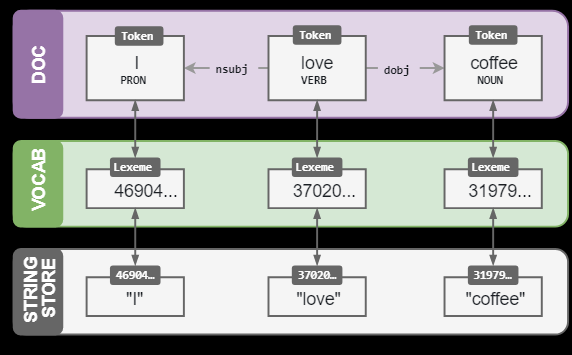
\includegraphics[width=0.5\linewidth,keepaspectratio]{spacy14}
\end{center}
	
\end{frame}

%%%%%%%%%%%%%%%%%%%%%%%%%%%%%%%%%%%%%%%%%%%%%%%%%%%%%%%%%%%%%%%%%%%%%%%%%%%%%%%%%%
\begin{frame}[fragile]\frametitle{Example}

\begin{lstlisting}
nlp = spacy.load("en_core_web_sm")
doc = nlp("I love coffee")
print(doc.vocab.strings["coffee"])  # 3197928453018144401
print(doc.vocab.strings[3197928453018144401])  # 'coffee'

3197928453018144401
coffee
\end{lstlisting}

  \begin{itemize}
    \item All strings are encoded, the entries in the vocabulary don't need to include the word text themselves. Instead, they can look it up in the StringStore via its hash value. 
		\item Each entry in the vocabulary, also called Lexeme, contains the context-independent information about a word. 
		\item For example, no matter if “love” is used as a verb or a noun in some context, its spelling and whether it consists of alphabetic characters won't ever change. Its hash value will also always be the same.
  \end{itemize}


\end{frame}

%%%%%%%%%%%%%%%%%%%%%%%%%%%%%%%%%%%%%%%%%%%%%%%%%%%%%%%%%%%%%%%%%%%%%%%%%%%%%%%%%%
\begin{frame}[fragile]\frametitle{Example}

\begin{lstlisting}
nlp = spacy.load("en_core_web_sm")
doc = nlp("I love coffee")
for word in doc:
    lexeme = doc.vocab[word.text]
    print(lexeme.text, lexeme.orth, lexeme.shape_, lexeme.prefix_, lexeme.suffix_,
            lexeme.is_alpha, lexeme.is_digit, lexeme.is_title, lexeme.lang_)
\end{lstlisting}

	\begin{center}
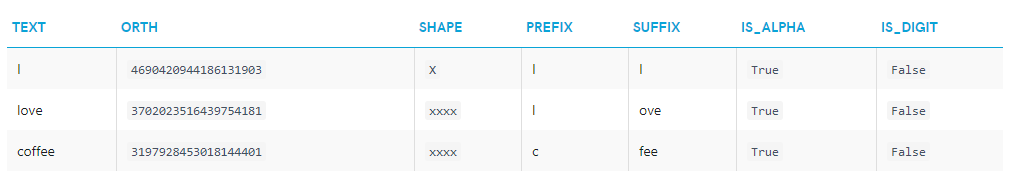
\includegraphics[width=\linewidth,keepaspectratio]{spacy15}
\end{center}


\end{frame}

%%%%%%%%%%%%%%%%%%%%%%%%%%%%%%%%%%%%%%%%%%%%%%%%%%%%%%%%%%%%%%%%%%%%%%%%%%%%%%%%%
\begin{frame}[fragile]\frametitle{Exercise}

  \begin{itemize}
    \item Look up the string “cat” in nlp.vocab.strings to get the hash.
    \item Look up the hash to get back the string.
  \end{itemize}
	
	
\begin{lstlisting}
from spacy.lang.en import English

nlp = English()
doc = nlp("I have a cat")

# Look up the hash for the word "cat"
cat_hash = ____.____.____[____]
print(cat_hash)

# Look up the cat_hash to get the string
cat_string = ____.____.____[____]
print(cat_string)
\end{lstlisting}




\end{frame}

%%%%%%%%%%%%%%%%%%%%%%%%%%%%%%%%%%%%%%%%%%%%%%%%%%%%%%%%%%%%%%%%%%%%%%%%%%%%%%%%%%
\begin{frame}[fragile]\frametitle{Official Help}
  \begin{itemize}
    \item Troubleshooting Guide https://spacy.io/usage/\#troubleshooting
		\item Github issues tracker https://github.com/explosion/spaCy/issues
		\item Stack Overflow  https://stackoverflow.com/questions/tagged/spacy
  \end{itemize}
	
	
\end{frame}